\documentclass{standalone}
\usepackage{pgfplots}

\begin{document}
\definecolor{ECG}{HTML}{ef6da1} 
\definecolor{EEG}{HTML}{60c5fd}
\definecolor{LFP}{HTML}{f2d1fe}
\definecolor{AP}{HTML}{5dc6a1}
\definecolor{EMG}{HTML}{986eec}
\begin{tikzpicture}
    \begin{axis}[
        grid=both, % Disable the grid
        axis lines=middle, % Draw x and y axis in the middle
        xmin=0, xmax=6, % Set x axis limits
        ymin=0, ymax=7, % Set y axis limits
        xtick={0, 1, 2, 3, 4, 5}, % Set positions of x ticks
        ytick={0, 1, 2, 3, 4, 5, 6}, % Set positions of y ticks
        xticklabels={$0$, $1$, $10$, $100$, $1k$, $10k$}, % Set labels of x ticks
        yticklabels={$0$, $100n$, $1\mu$, $10\mu$, $100\mu$, $1m$, $10m$}, % Set labels of y ticks
        x label style={at={(axis description cs:0.5,-0.1)},anchor=north},
        y label style={at={(axis description cs:-0.15,.5)},rotate=90,anchor=south},
        xlabel={Frequency $[Hz]$},
        ylabel={Amplitude $[V]$}
    ]
    \draw [rounded corners, fill=ECG, opacity=0.6] (axis cs:1,4.5) rectangle (axis cs:4,5.7);
    \node at (axis cs:1.5, 5.3) {ECG};

    \node[inner sep=0pt] (heart) at (axis cs:0.5,5.1)
    {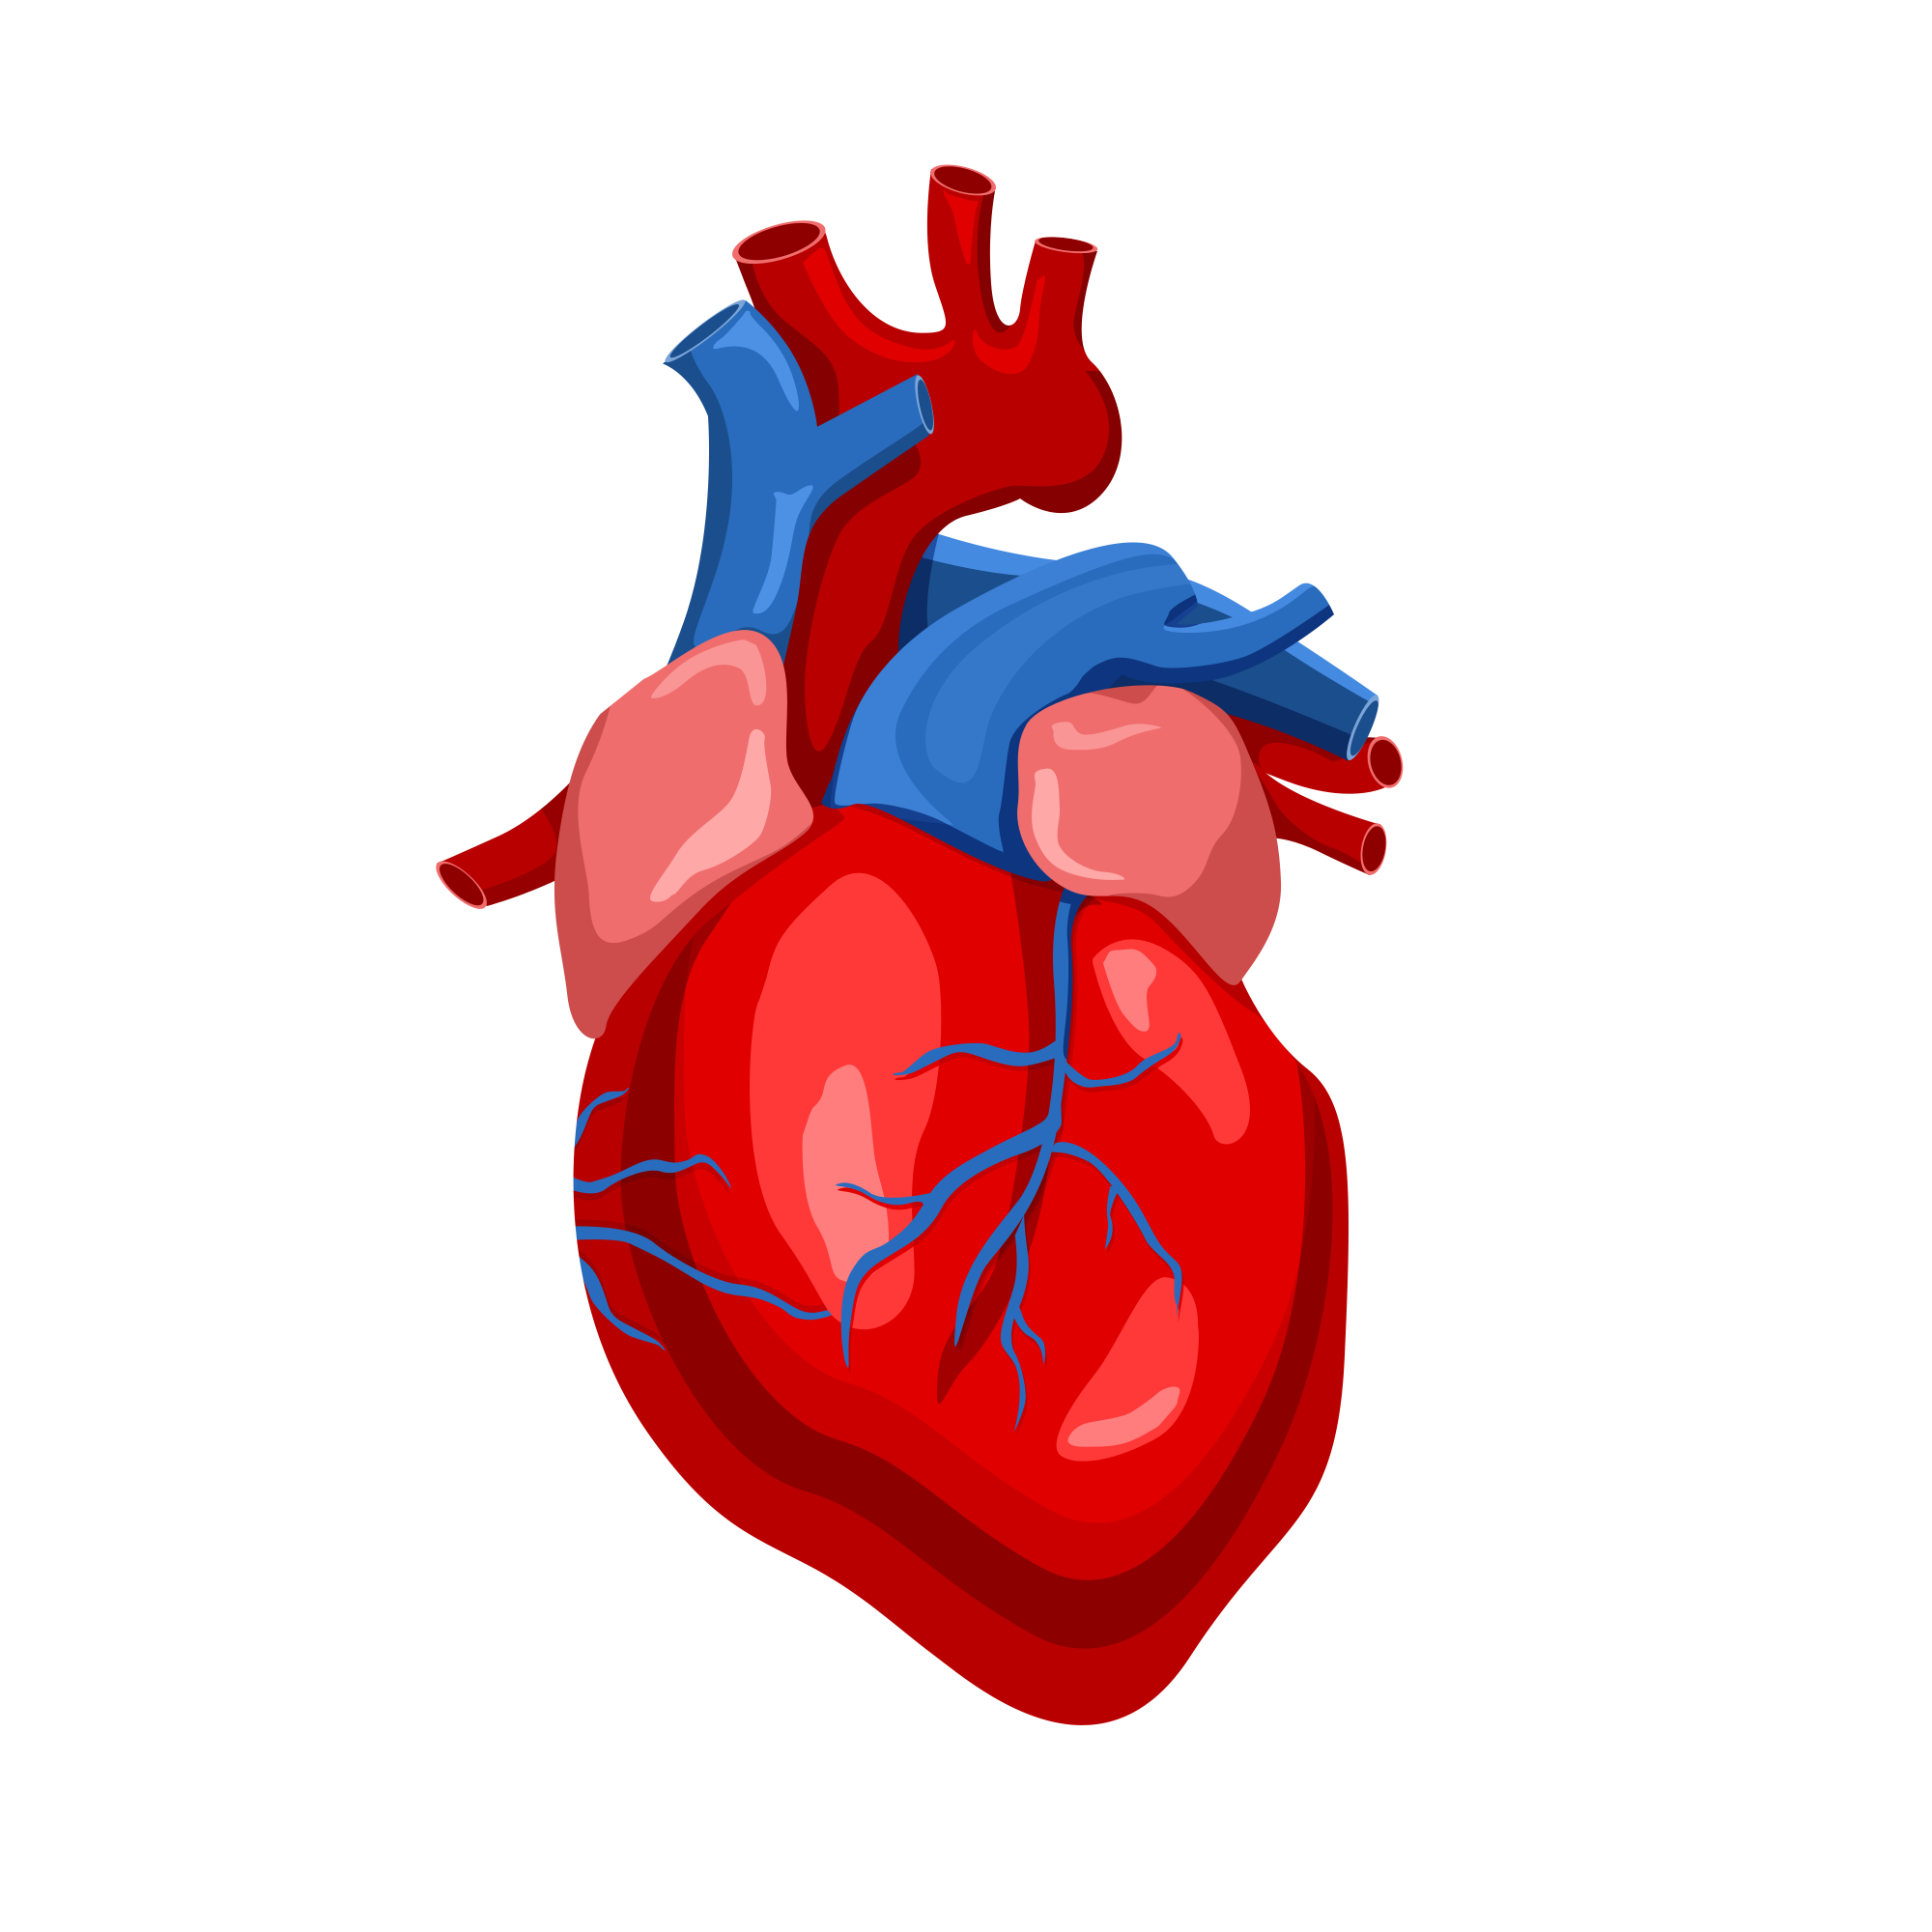
\includegraphics[width=.12\textwidth]{img/heart.png}};
    
    \draw [rounded corners, fill=AP, opacity=0.6] (axis cs:3.1,3.1) rectangle (axis cs:5,5);
    \node at (axis cs:4.5, 4.2) {AP};
    
    \draw [rounded corners, fill=EEG, opacity=0.8] (axis cs:1,2) rectangle (axis cs:3.2,3.2);
    \node at (axis cs:2.1, 2.6) {EEG};

    \node[inner sep=0pt] (brain) at (axis cs:1.5,1.2)
    {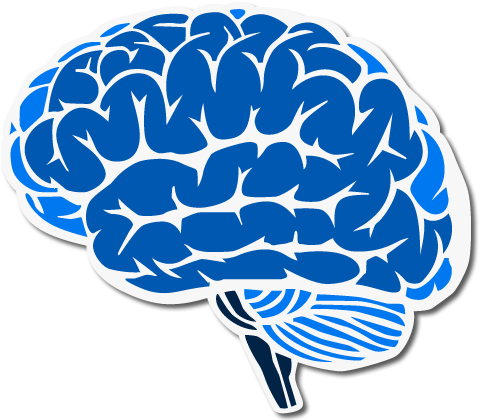
\includegraphics[width=.1\textwidth]{img/brain.png}};

    \draw [rounded corners, fill=LFP, opacity=0.4] (axis cs:1,3) rectangle (axis cs:3.5,5);
    \node at (axis cs:1.5, 4) {LFP};

    \draw [rounded corners, fill=EMG, opacity=0.6] (axis cs:2,3.2) rectangle (axis cs:4,5.4);
    \node at (axis cs:3, 5.2) {EMG};

    \node[inner sep=0pt] (brain) at (axis cs:3,6.25)
    {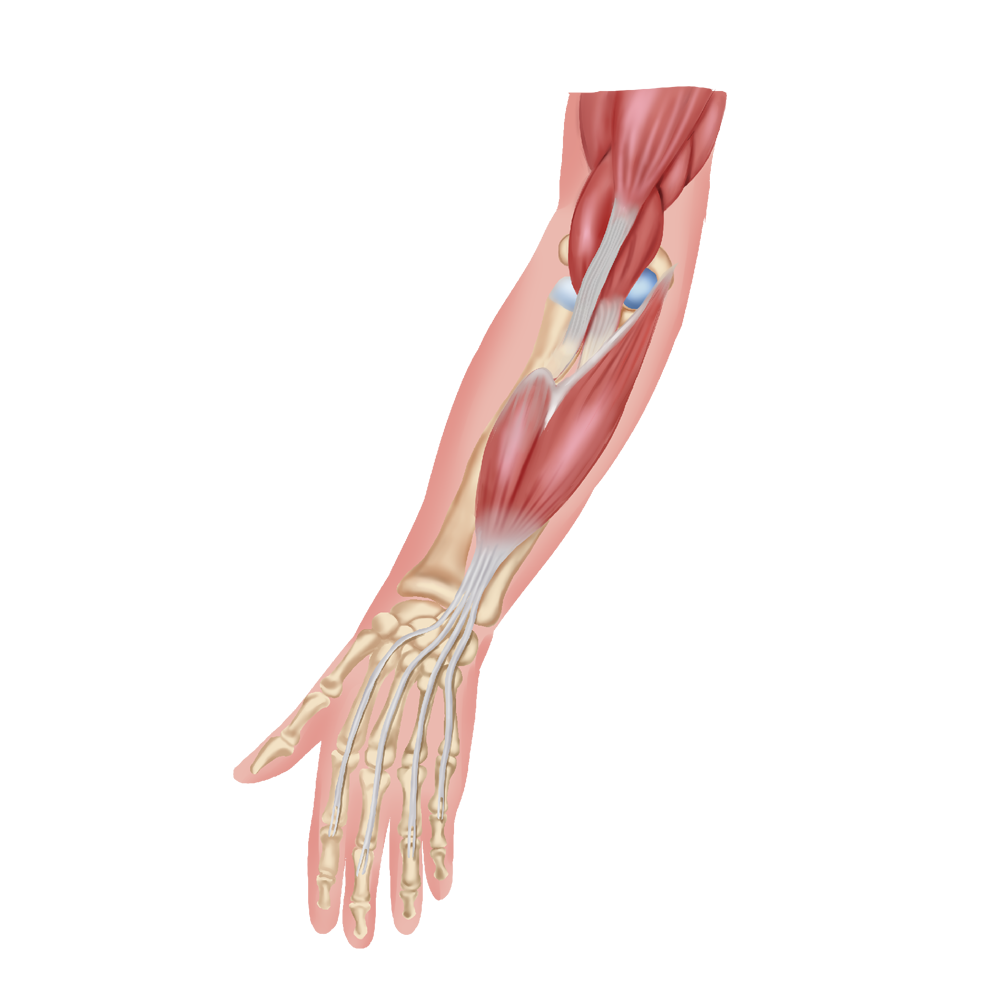
\includegraphics[width=.2\textwidth,angle=-70,origin=c]{img/muscle.png}};
    \end{axis}
\end{tikzpicture}
\end{document}